\subsection{Tracing backend}

\begin{frame}{Tracing}
\begin{exampleblock}{}
  {``Tracing is a specialized use of logging to record information about a
program's execution''}
  \vskip5mm
  \hspace*\fill{\small Wikipedia}
\end{exampleblock}
\hfill \\
\hfill \\
Tracing characteristics:
\begin{itemize}
\item Tracing can be low level (eg. kernel tracing, access to performance
counters)
\item Tracing has mostly debugging purposes and performance tuning
\item Tracing may produce notoriously bulky output
\end{itemize}
\end{frame}

\begin{frame}{Tracing Systems}
\setbeamertemplate{description item}[align left]
\begin{description}
\item[DTrace] \hfill \\
Released by Sun Microsystems in 2005
\item[SystemTap] \hfill \\
Released by Red Hat in 2005
\end{description}

Advantages:
\begin{itemize}
\item Dynamic Instrumentation
\item User and kernel tracing
\end{itemize}

\hfill \\
Disadvantages:
\begin{itemize}
\item User tracing is based or system calls or breakpoints
\item Significant performance overhead
\item Inappropriate for live tracing
\end{itemize}
\end{frame}

\begin{frame}{Linux Trace Toolkit - next generation}

\includegraphics[scale=0.08]{images/lttng-logo.png}
\begin{itemize}
\item successor of Linux Trace Toolkit
\item Mathieu Desnoyers' PhD dissertation  in École Polytechnique de Montréal
\item maintained by EfficiOS Inc and the DORSAL lab in École Polytechnique de
Montréal.
\item Unified user and kernel tracing
\item Low overhead tracing based on Tracepoints
\item Static instrumentation
\item Live tracing
\end{itemize}
\end{frame}

\subsection{LTTng}

\begin{frame}{LTTng Unified Tracing}
\begin{center}
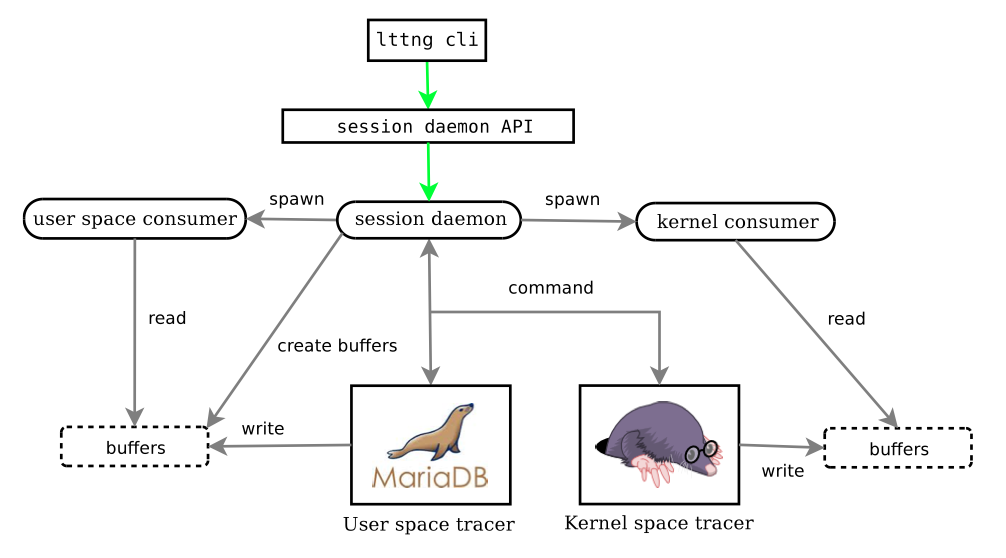
\includegraphics[scale=0.3]{images/lttng-arch.png}
\end{center}
\end{frame}

\begin{frame}{UST architecture}
\begin{center}
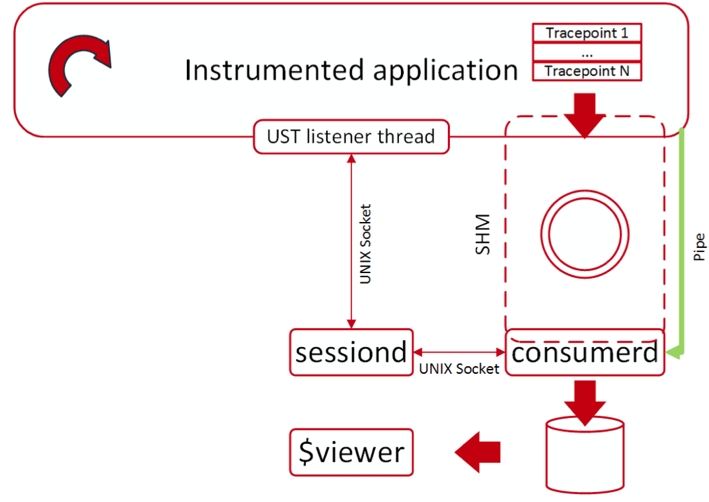
\includegraphics[scale=0.5]{images/ust-architecture.png}
\end{center}
\end{frame}

\begin{frame}{LTTng live-tracing}
\begin{center}
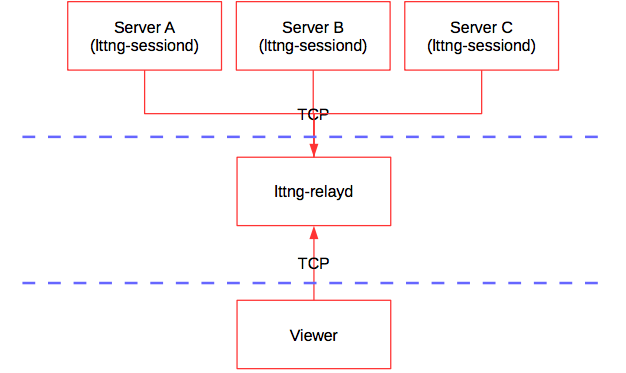
\includegraphics[scale=0.4]{images/relayd.png}
\end{center}
\end{frame}

\begin{frame}{CTF}
Common Trace Format:
\hfill \\
\begin{itemize}
\item Aimed to cover tracing needs from versatile communities
\item Collaboration between the Multicore association and the Linux Community
\item Based on Trace Stream Description Language
\item Separation between data and metadata
\item Separation between event and event-context
\item Variety of data types and type inheritance
\item Live tracing
\end{itemize}
\end{frame}

\begin{frame}{Babeltrace}
\begin{itemize}
\item Trace reader/writer
\item Trace converter
\item Babeltrace plugins
\item Exports \texttt{libbabeltrace}
\item Python bindings
\end{itemize}
\hfill \\
\hfill \\
Complete environments based on Babeltrace: Trace Compass (Java tool), Eclipse
LTTng plugin
\end{frame}
